\documentclass[a4paper]{article}

\usepackage[english]{babel}
\usepackage[utf8]{inputenc}
\usepackage{amsmath}
\usepackage{graphicx}
\usepackage{epsfig}
\usepackage{amsfonts}
\usepackage[ruled,vlined]{algorithm2e}
\usepackage{bbm}
\usepackage{pythonhighlight}
\usepackage[colorinlistoftodos]{todonotes}
\usepackage[hidelinks]{hyperref}
\usepackage[margin=1.3in]{geometry}

\DeclareMathOperator*{\argmax}{arg\,max}
\DeclareMathOperator*{\argmin}{arg\,min}

\title{Object Detection Reviews}

\author{Ao Zhang}

%\date{June 2015}

\newcommand{\gfigure}[4]
{
	\begin{figure}
      \begin{center}
          \includegraphics[#3]{#4}
          \caption{#1}
          \label{Figure:#2}
      \end{center}
    \end{figure}
}
\newcommand{\figref}[1]{Figure~\ref{Figure:#1}}

\begin{document}
\maketitle


%\begin{figure}[h]
%	\centering
%	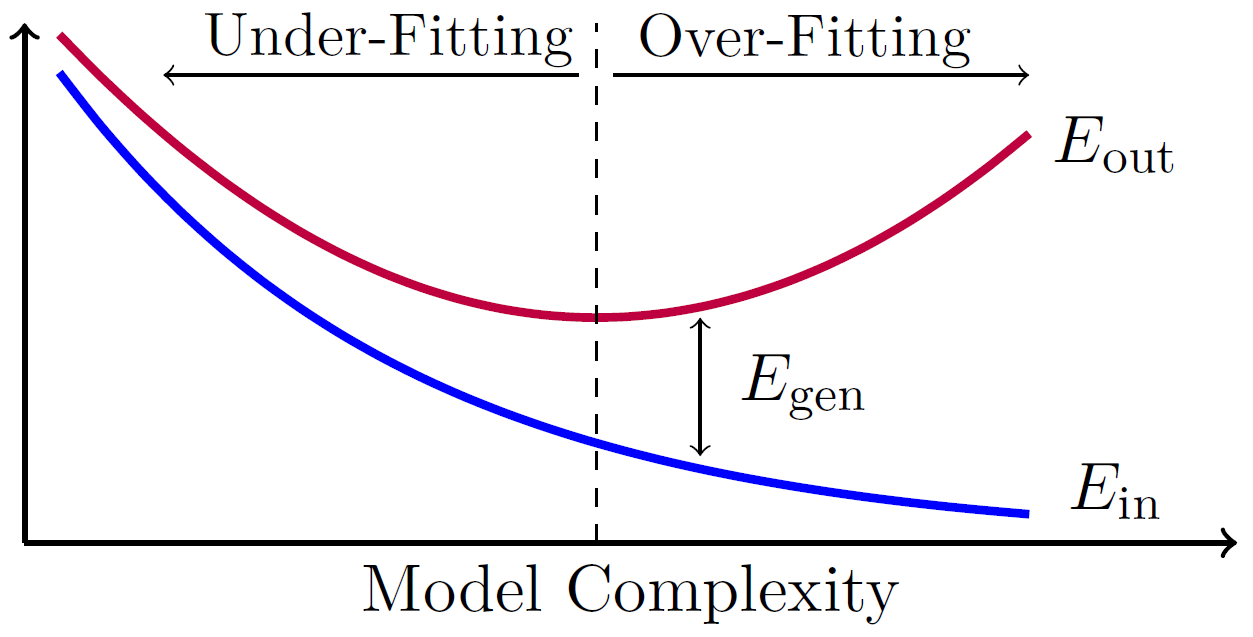
\includegraphics[width=0.6\textwidth]{images/overfitting.png}
%	\caption{Overfitting and Underfitting}
%	\label{fig:mesh1}
%\end{figure}



%%%%%%%%%%%%%%%%%%%%%%%%%%%%%%%% Starting here, we shall write another one %%%%%%%%%%%%%%%%%%%%%%%%%%%%%%%

\section{Backbones}

\begin{itemize}
	\item \textbf{Xception}
	\item \textbf{VGG16}
	\item \textbf{ResNet50}
	\item \textbf{InceptionV3}
	\item \textbf{MobileNet}
	\item \textbf{DenseNet}
	\item \textbf{NASNet}
\end{itemize}

\section{Neck Layers}

\begin{itemize}
	\item \textbf{Feature Pyramid Networks (FPN)}
\end{itemize}


\section{Detection Head}

\subsection{One-Stage Detector}

\begin{itemize}
	\item \textbf{YOLO}: The final feature maps shape of YOLO Detection Head should be $(B, W, H, K \times (5 + num\_classes))$, where $K$ means number of anchor boxes; $5$ including box info $[x, y, w, h]$ and an ``objectness''. The box decoding system is shown as below.
	\begin{figure}[h]
		\centering
		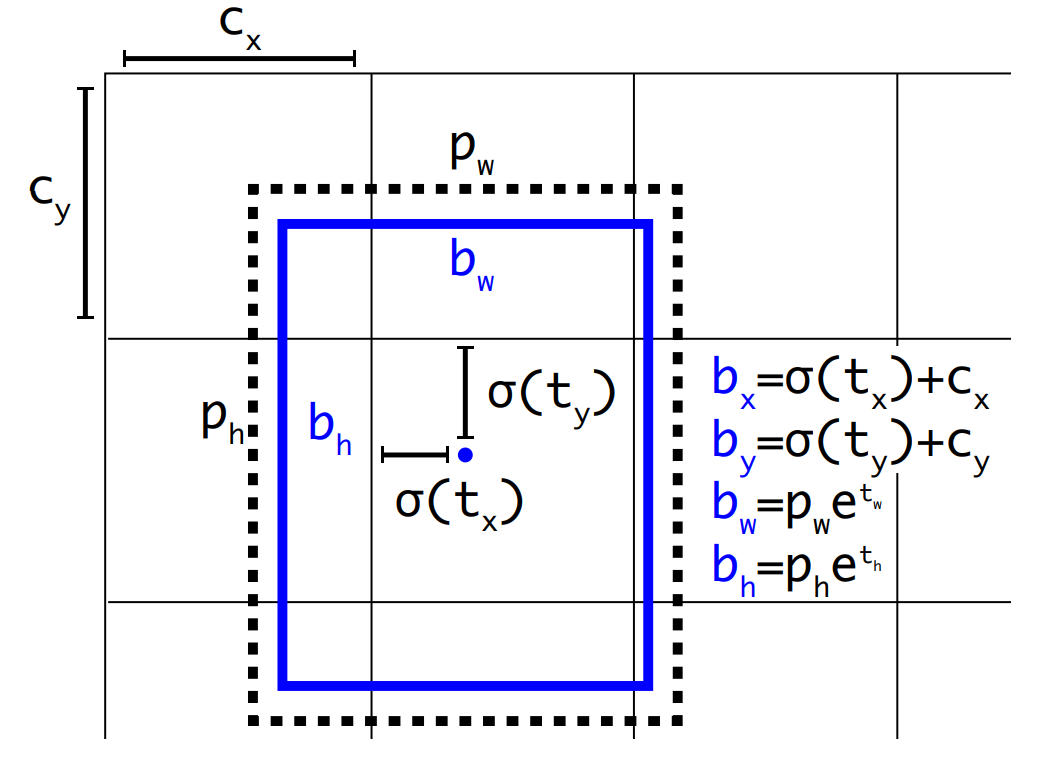
\includegraphics[width=0.5\textwidth]{images/YOLO.png}
		\caption{YOLO}
		\label{fig:yolo}
	\end{figure}
	The anchor boxes of YOLO are directly found by K-means Clustering on the entire dataset with a certain error rate threshold.
	\item \textbf{SSD}: The final feature maps shape of SSD Detection Head should be $(B, m, W, H, K \times (4 + num\_classes))$, where $m$ means number of output feature layers for the decoding; $4$ consist $[x, y, w, h]$. The box decoding system is shown as below.
	\begin{figure}[h]
		\centering
		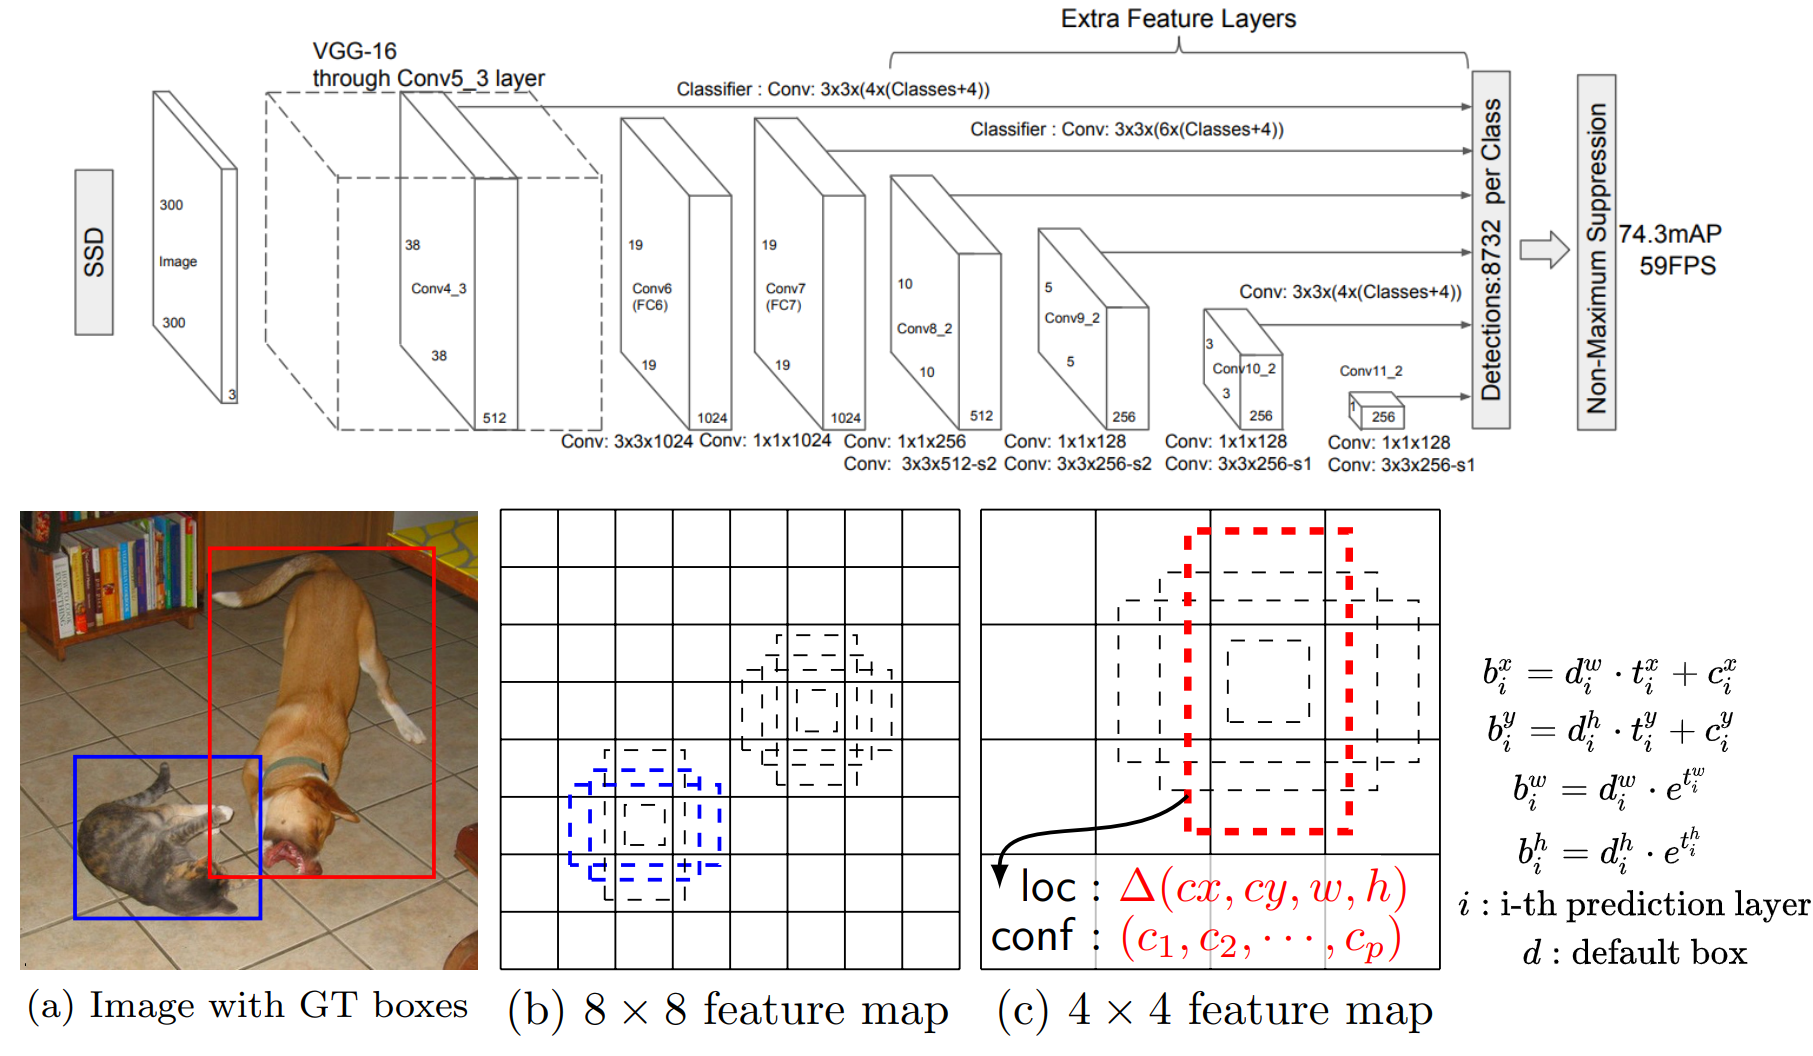
\includegraphics[width=0.9\textwidth]{images/SSD.png}
		\caption{SSD}
		\label{fig:ssd}
	\end{figure}
	The anchor boxes of SSD is a little different. It first defines box aspect ratios with K-means Clustering. Then define the boxes with scales $s$ and aspect ratios $a_r$. 
	\begin{align}
		s_k &= s_{min} + \frac{s_{max} - s_{min}}{m -1}(k - 1),\,\,\,\, k \in [1, m] \\
		w_k^a &= s_k \sqrt{a_r},\,\,\,\, h_k^a = s_k / \sqrt{a_r} \\
		a_R &\in \{ 1, 2, 3, \frac{1}{2}, \frac{1}{3} \}
	\end{align}
	Where, $m$ is the total number of output feature layers. For the default box, it is defined with scale $s_k^{\prime} = \sqrt{s_k s_{k+1}}$.
	On the other hand, since SSD doesn't have ``objectness''. The \textbf{hard negative mining} is required for training. Hard negative mining is to select the negative samples with highest prediction probilities to conduct backpropagation. In SSD itself, the ratio of negative samples to positive samples is ensured as $3:1$.
\end{itemize}

\subsection{Two-Stage Detector}

\begin{itemize}
	\item \textbf{Faster R-CNN}: \textbf{Region Proposal Networks} + \textbf{Classification Head}; It is an anchor-based method.
\end{itemize}

\section{Metrics}

\begin{itemize}
	\item \textbf{Precision}:
	\begin{equation}
		\text{precision} = \frac{TP}{TP + FP}
	\end{equation}
	\item \textbf{Recall}:
	\begin{equation}
		\text{recall} = \frac{TP}{TP + FN}
	\end{equation}
	\item \textbf{Average Precision (AP)}: the area of precision-recall curves.
	\item \textbf{F1 Score}:
	\begin{equation}
		F1 = \frac{2}{\frac{1}{\text{precision}} + \frac{1}{\text{recall}}} = \frac{TP}{TP + \frac{FN + FP}{2}}
	\end{equation}
	\item \textbf{Receiver Operating Characteristics (ROC) Curves}:
	\begin{align}
		TPR &= \frac{TP}{TP + FN} \\
		FPR &= \frac{FP}{TN + FP}
	\end{align}
	\item \textbf{Confusion Matrix}: assume a classification task, the confusion matrix is computed on the validation set with each entry of the matrix indicating the count for each class predicted by the classifier. Example shown as below.
	\begin{equation}
		C = 
		\begin{bmatrix}
			21 & 2 & 7 \\
			10 & 11 & 9 \\
			3 & 1 & 26 \\
		\end{bmatrix}
	\end{equation}
	Where, the perfect classifier would have results like,
	\begin{equation}
		C = 
		\begin{bmatrix}
			30 & 0 & 0 \\
			0 & 30 & 0 \\
			0 & 0 & 30 \\
		\end{bmatrix}
	\end{equation}
\end{itemize}

\section{Others}

\subsection{Data Augmentation}

\begin{itemize}
	\item \textbf{Point Operations}: Change brightness, saturation, hue, gamma, correction, histogram equalization, etc.
	\item \textbf{Geometric Operations}: Shift, flip, rotate or shear.
	\item \textbf{Adding Noise}: Gaussian noise, etc.
\end{itemize}

\subsection{Loss Functions}

\subsection{Regularization}

\subsection{Normalization}

\subsection{Skip-Connections}

%%%%%%%%%%%%%%%%%%%%%%%%%%%%%%%%%%%%%%%%%%%%%%%%%%%%%%%%%%%%%%%%%%%%%%%%%%%%%%%%%%%%%%%%%%%%%%%%%


%\bibliographystyle{acm}
%\bibliography{bibliography}
\end{document}